\documentclass{article}
\usepackage{amsmath}
\usepackage{graphicx}
\usepackage{lipsum}

\title{Detailed Explanations of Macroeconomic Concepts}
\author{Charles Ancel}
\date{July 3, 2024}

\begin{document}

\maketitle

\section{Introduction}
My name is Charles Ancel, my UIN is 654604114, and this is my ID. I'm currently
enrolled in ECON 425 during the Summer Session and I understand that this
assignment is part of the requirement from the University regarding the College
of LAS's identity verification policy for LAS Online-certified classes. For the
answers in this assignment, I did not use any form of Artificial Intelligence (AI)
help, such as Chat-GPT or similar, and thus my answers will accurately and fairly
reflect my own learning from this course.

\hrulefill

\section{Relationship Between Real and Nominal Interest Rates and Their Effect on Consumption}

\textbf{Question 1:} What is the exact relationship between the real and the nominal interest rates? How does the real interest rate affect consumption?

\textbf{1.1 Nominal Interest Rate:} The nominal interest rate is the stated interest rate on a loan or investment, not adjusted for inflation. It represents the percentage increase in money that a borrower pays to a lender. For example, if you have a savings account with a nominal interest rate of 5\%, you will receive 5\% of your balance as interest over a year.

\textbf{1.2 Real Interest Rate:} The real interest rate adjusts the nominal rate to remove the effects of inflation and represents the true cost of borrowing and the real yield on an investment. The formula is:

\begin{equation*}
    \text{Real Interest Rate} = \text{Nominal Interest Rate} - \text{Inflation Rate}
\end{equation*}

For example, if the nominal interest rate is 5\% and the inflation rate is 2\%, the real interest rate is 3\%. This 3\% reflects the actual increase in purchasing power from saving.

\textbf{1.3 Effect on Consumption:} Low real interest rates make borrowing cheaper, which encourages households to take out loans for consumption (e.g., buying cars or houses) and investment. This increases overall consumer spending in the economy. Conversely, high real interest rates make borrowing more expensive, discouraging households from taking out loans. Instead, they are more likely to save money, reducing their current spending. This leads to lower overall consumption in the economy.

\textbf{Graph: Real and Nominal Interest Rates:} 

To visualize the relationship between real and nominal interest rates, we plot both rates over time. The blue line represents the nominal interest rate, while the red line represents the real interest rate. This graph helps us understand how inflation impacts the real interest rate, showing the difference between what is nominally earned and what is actually gained in terms of purchasing power.

\begin{figure}[h!]
    \centering
    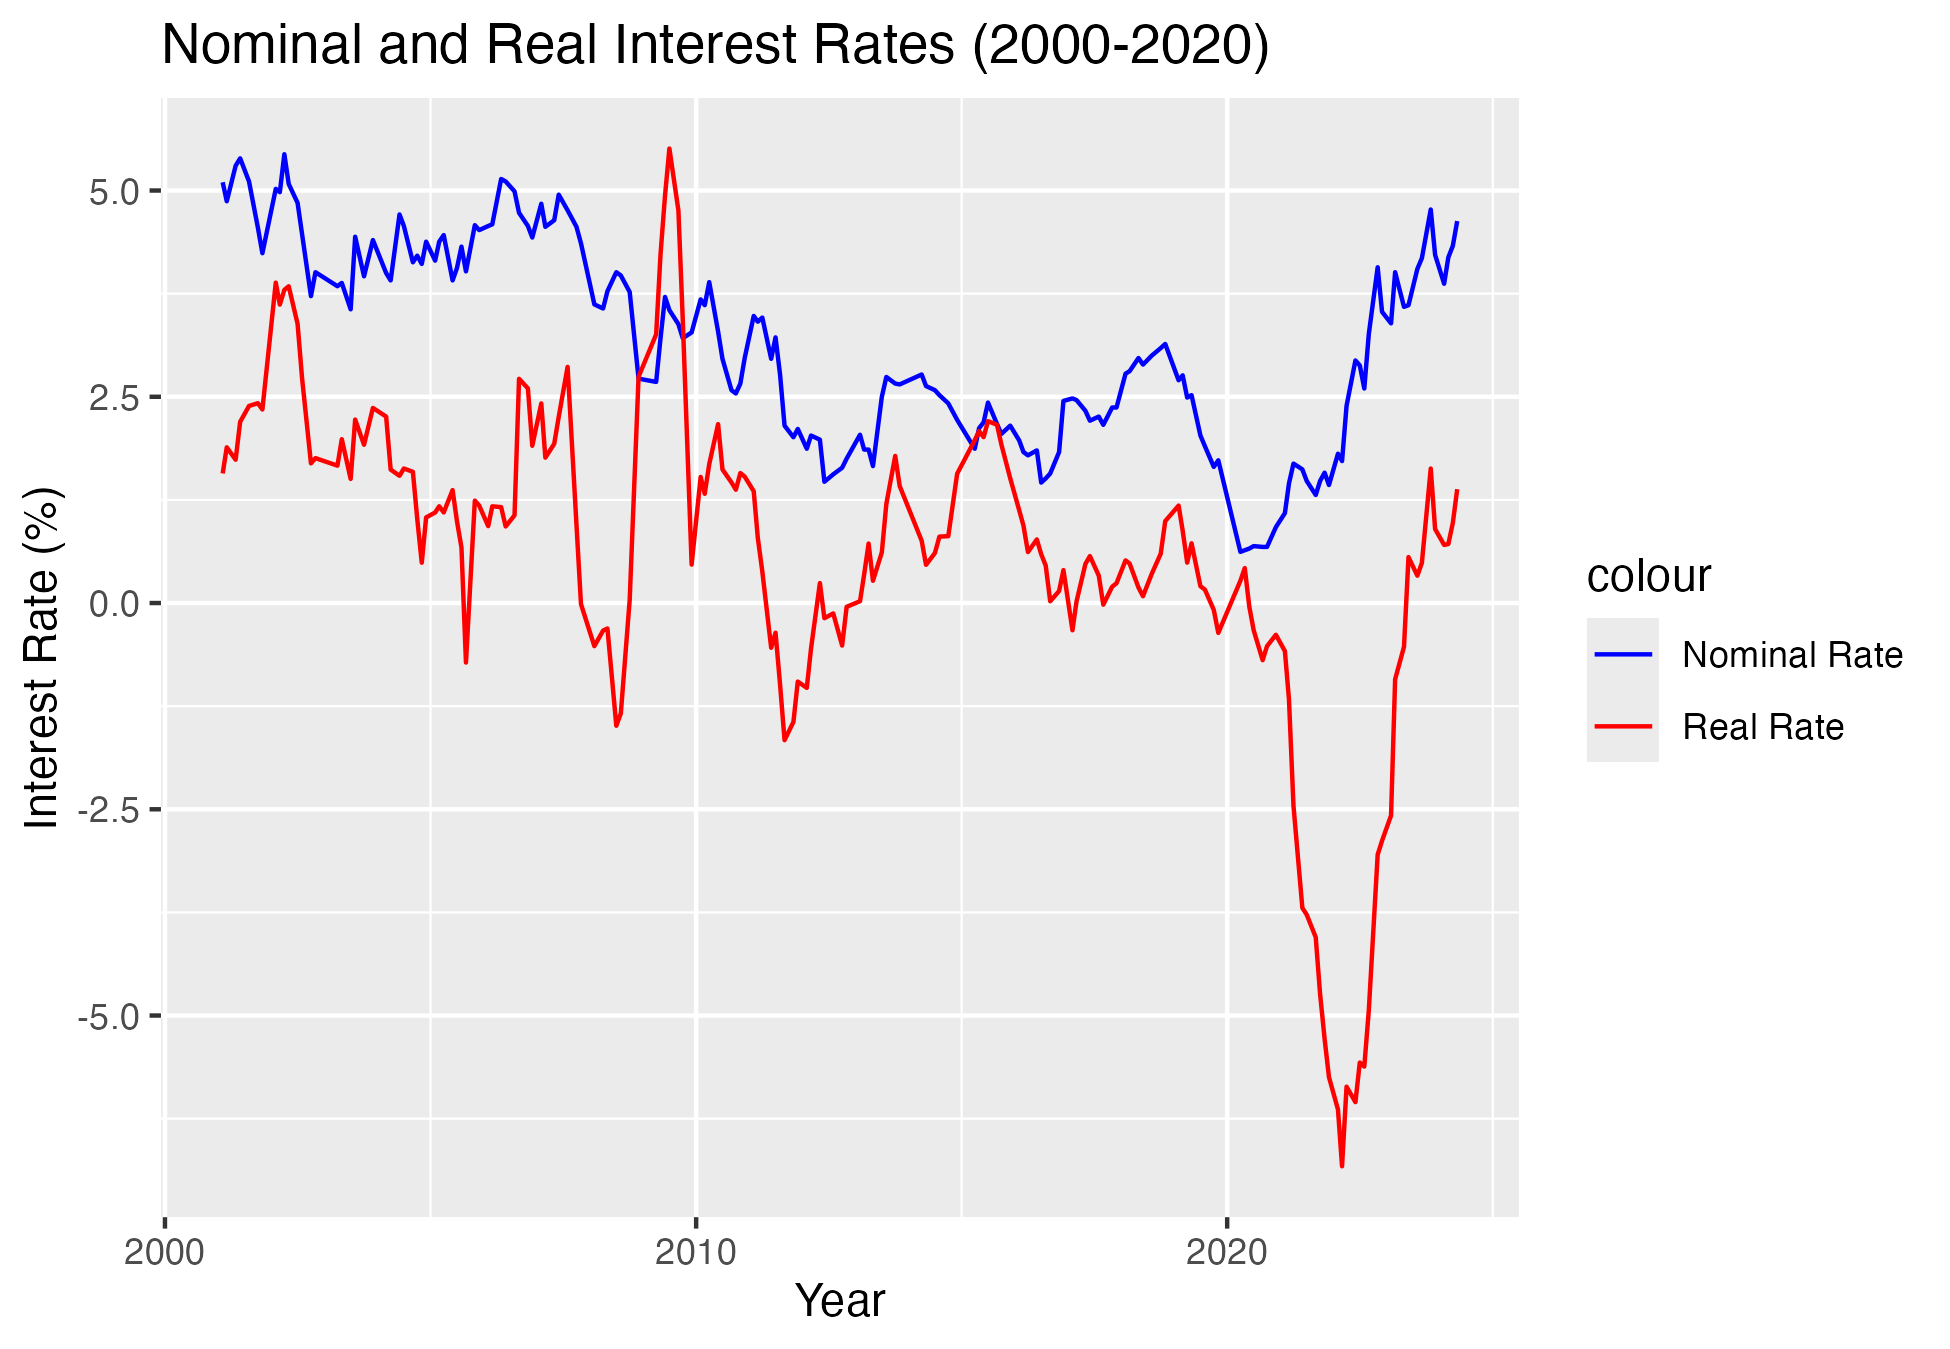
\includegraphics[width=0.9\textwidth]{/Users/cancel/Personal/Coursework/Econ425/VA1/R/Nominal_vs_Real_Interest_Rates.png}
    \caption{Real and Nominal Interest Rates}
\end{figure}

\hrulefill

\section{Debt Constraints and Policy Decisions}

\textbf{Question 2:} Should we base our policy decisions on assuming no consumer faces debt constraints? Why, and what are the consequences of doing so?

\textbf{2.1 Debt Constraints:} Debt constraints refer to the limitations faced by consumers in their ability to borrow money. These constraints can arise due to lack of collateral, poor credit history, or high levels of existing debt. Many households cannot borrow as much as they would like, which affects their consumption and savings decisions.

\textbf{2.2 Assuming No Debt Constraints:} Policies based on the assumption that consumers are not debt-constrained may overestimate the impact of fiscal or monetary measures. For instance, tax cuts or interest rate reductions might not lead to the expected increase in consumption if many households cannot borrow due to debt constraints. If policy decisions ignore debt constraints, they might not provide adequate support to constrained households, leading to ineffective policy measures, increased inequality, and economic instability. For example, during a recession, if debt-constrained households cannot increase their consumption despite lower interest rates, the economy might not recover as quickly as anticipated.

\textbf{Graph: Total Consumer Credit:} 

To understand the impact of debt constraints, we plot the total consumer credit over time. This graph shows the trend of consumer borrowing and helps illustrate the extent to which households rely on credit. A rising trend in consumer credit indicates increasing borrowing, while a declining trend may suggest tightening credit conditions or higher debt constraints.

\begin{figure}[h!]
    \centering
    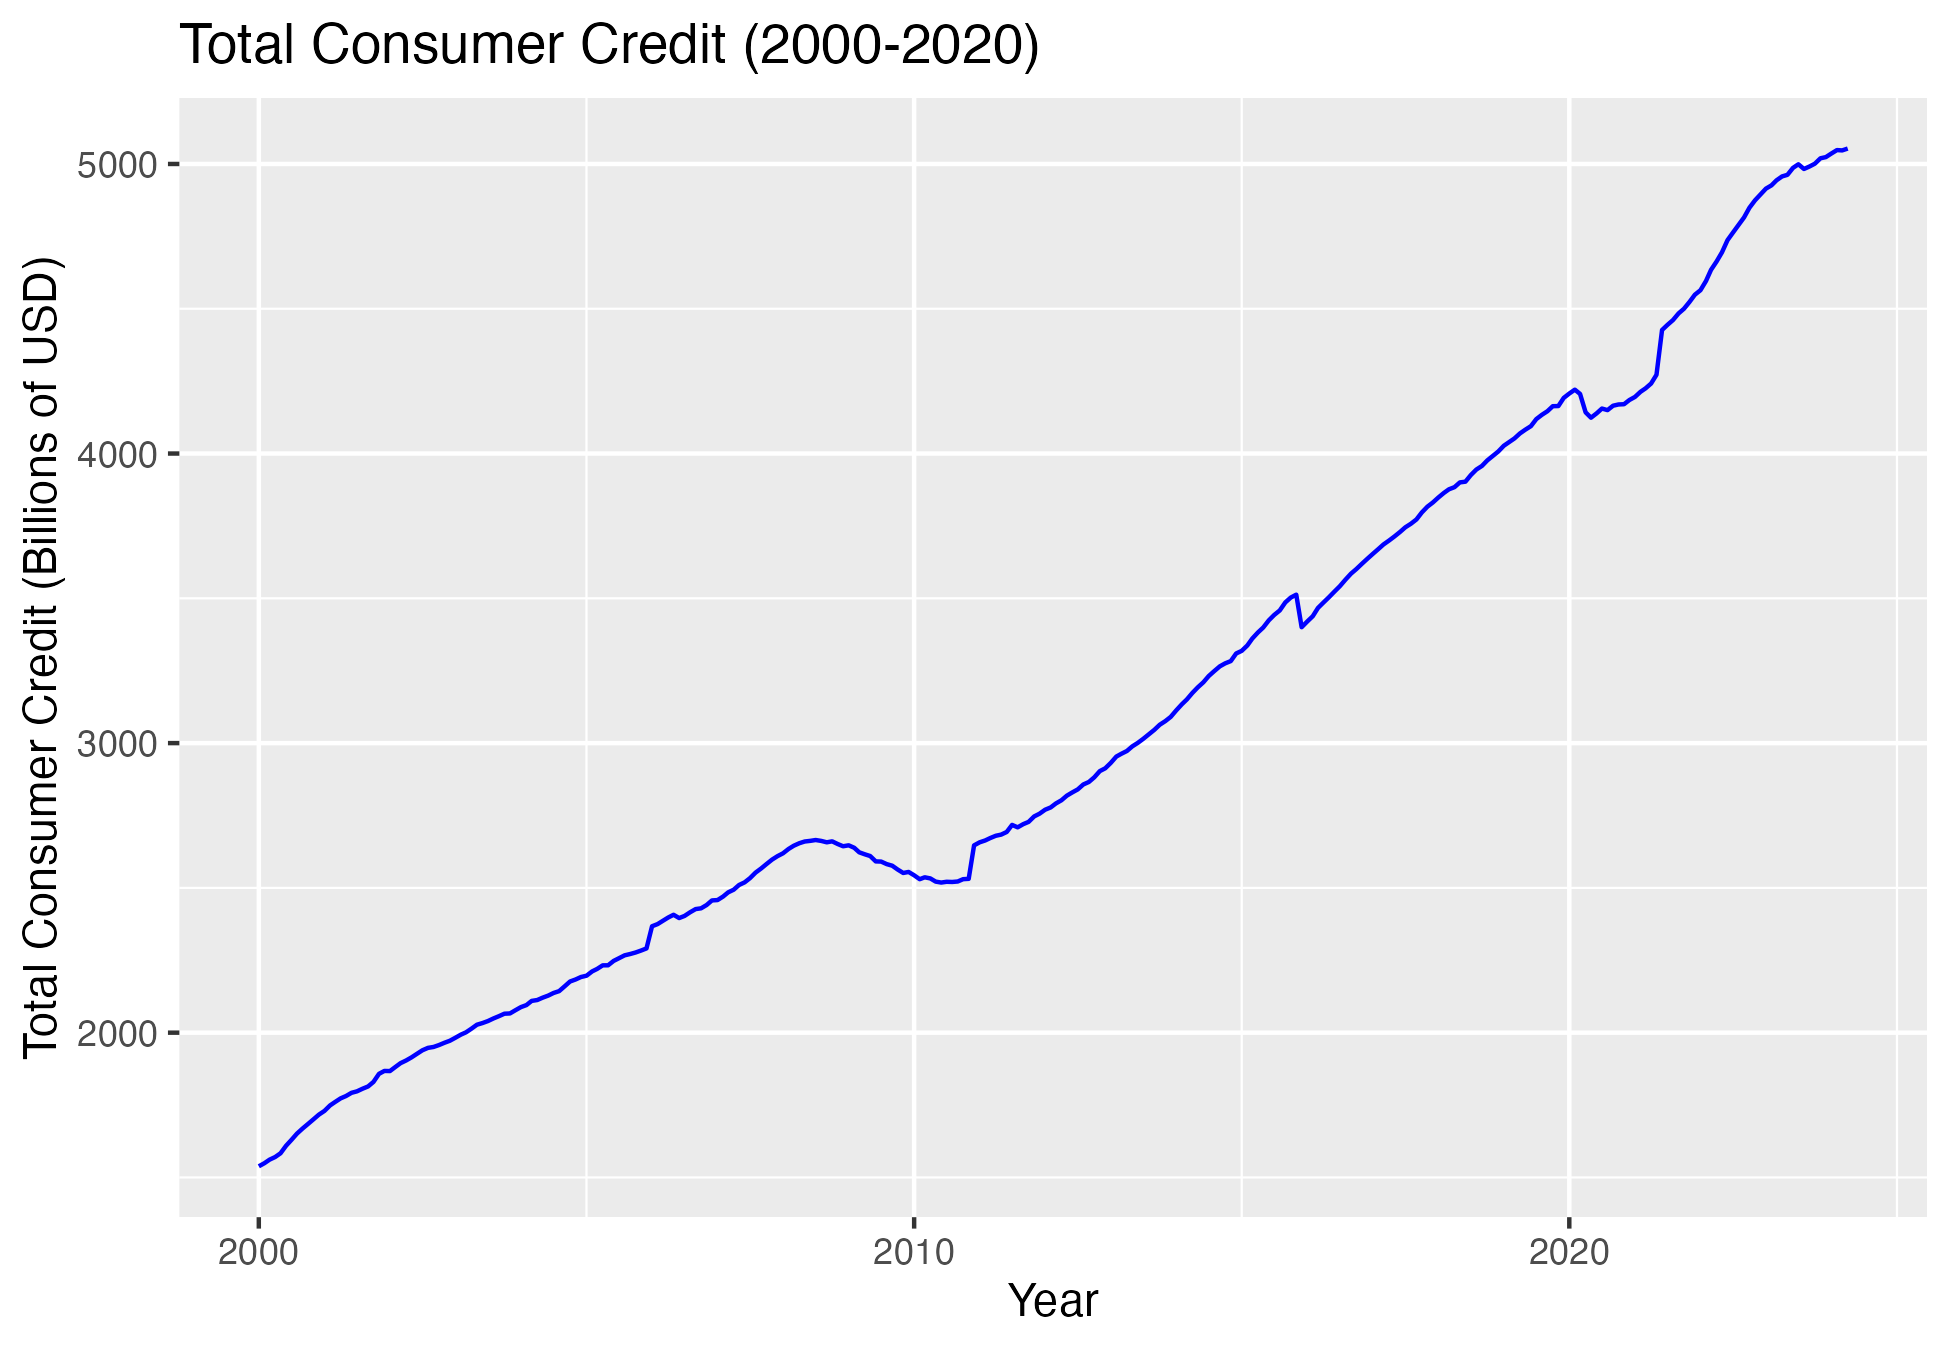
\includegraphics[width=0.9\textwidth]{/Users/cancel/Personal/Coursework/Econ425/VA1/R/Total_Consumer_Credit.png}
    \caption{Total Consumer Credit}
\end{figure}

\hrulefill

\section{Determinants of Nominal and Real Exchange Rates}

\textbf{Question 3:} In the short run, what is the main determinant of the nominal and real exchange rates? What is the role of the Uncovered Interest Rate Parity (UIP)?

\textbf{3.1 Nominal Exchange Rate:} The nominal exchange rate is the rate at which one currency can be exchanged for another. For example, if 1 US dollar can be exchanged for 110 Japanese yen, the nominal exchange rate is 110 yen per dollar. This rate is influenced by factors such as interest rates, inflation rates, and expectations of future exchange rates.

\textbf{3.2 Real Exchange Rate:} The real exchange rate adjusts the nominal exchange rate for differences in price levels between two countries and reflects the relative purchasing power of two currencies. The formula is:

\begin{align*}
    \text{Real Exchange Rate} = \frac{\text{Nominal Exchange Rate} \times \text{Domestic Price Level}}{\text{Foreign Price Level}}
\end{align*}

For example, if the nominal exchange rate is 110 yen per dollar, the domestic price level is 100, and the foreign price level is 90, the real exchange rate is approximately 122.22.

\textbf{3.3 Uncovered Interest Rate Parity (UIP):} Uncovered Interest Rate Parity (UIP) suggests that the difference in interest rates between two countries should equal the expected change in exchange rates between those countries’ currencies. If one country has a higher interest rate, its currency is expected to depreciate relative to a country with a lower interest rate. UIP helps explain why exchange rates move as they do, based on interest rate differentials.

\textbf{Graph: Nominal Exchange Rate and Interest Rate Differential:} 

This graph illustrates the relationship between the nominal exchange rate and the interest rate differential between two countries. The blue line represents the nominal exchange rate, while the red line shows the interest rate differential. This visual helps us understand how differences in interest rates can influence exchange rate movements.

\begin{figure}[h!]
    \centering
    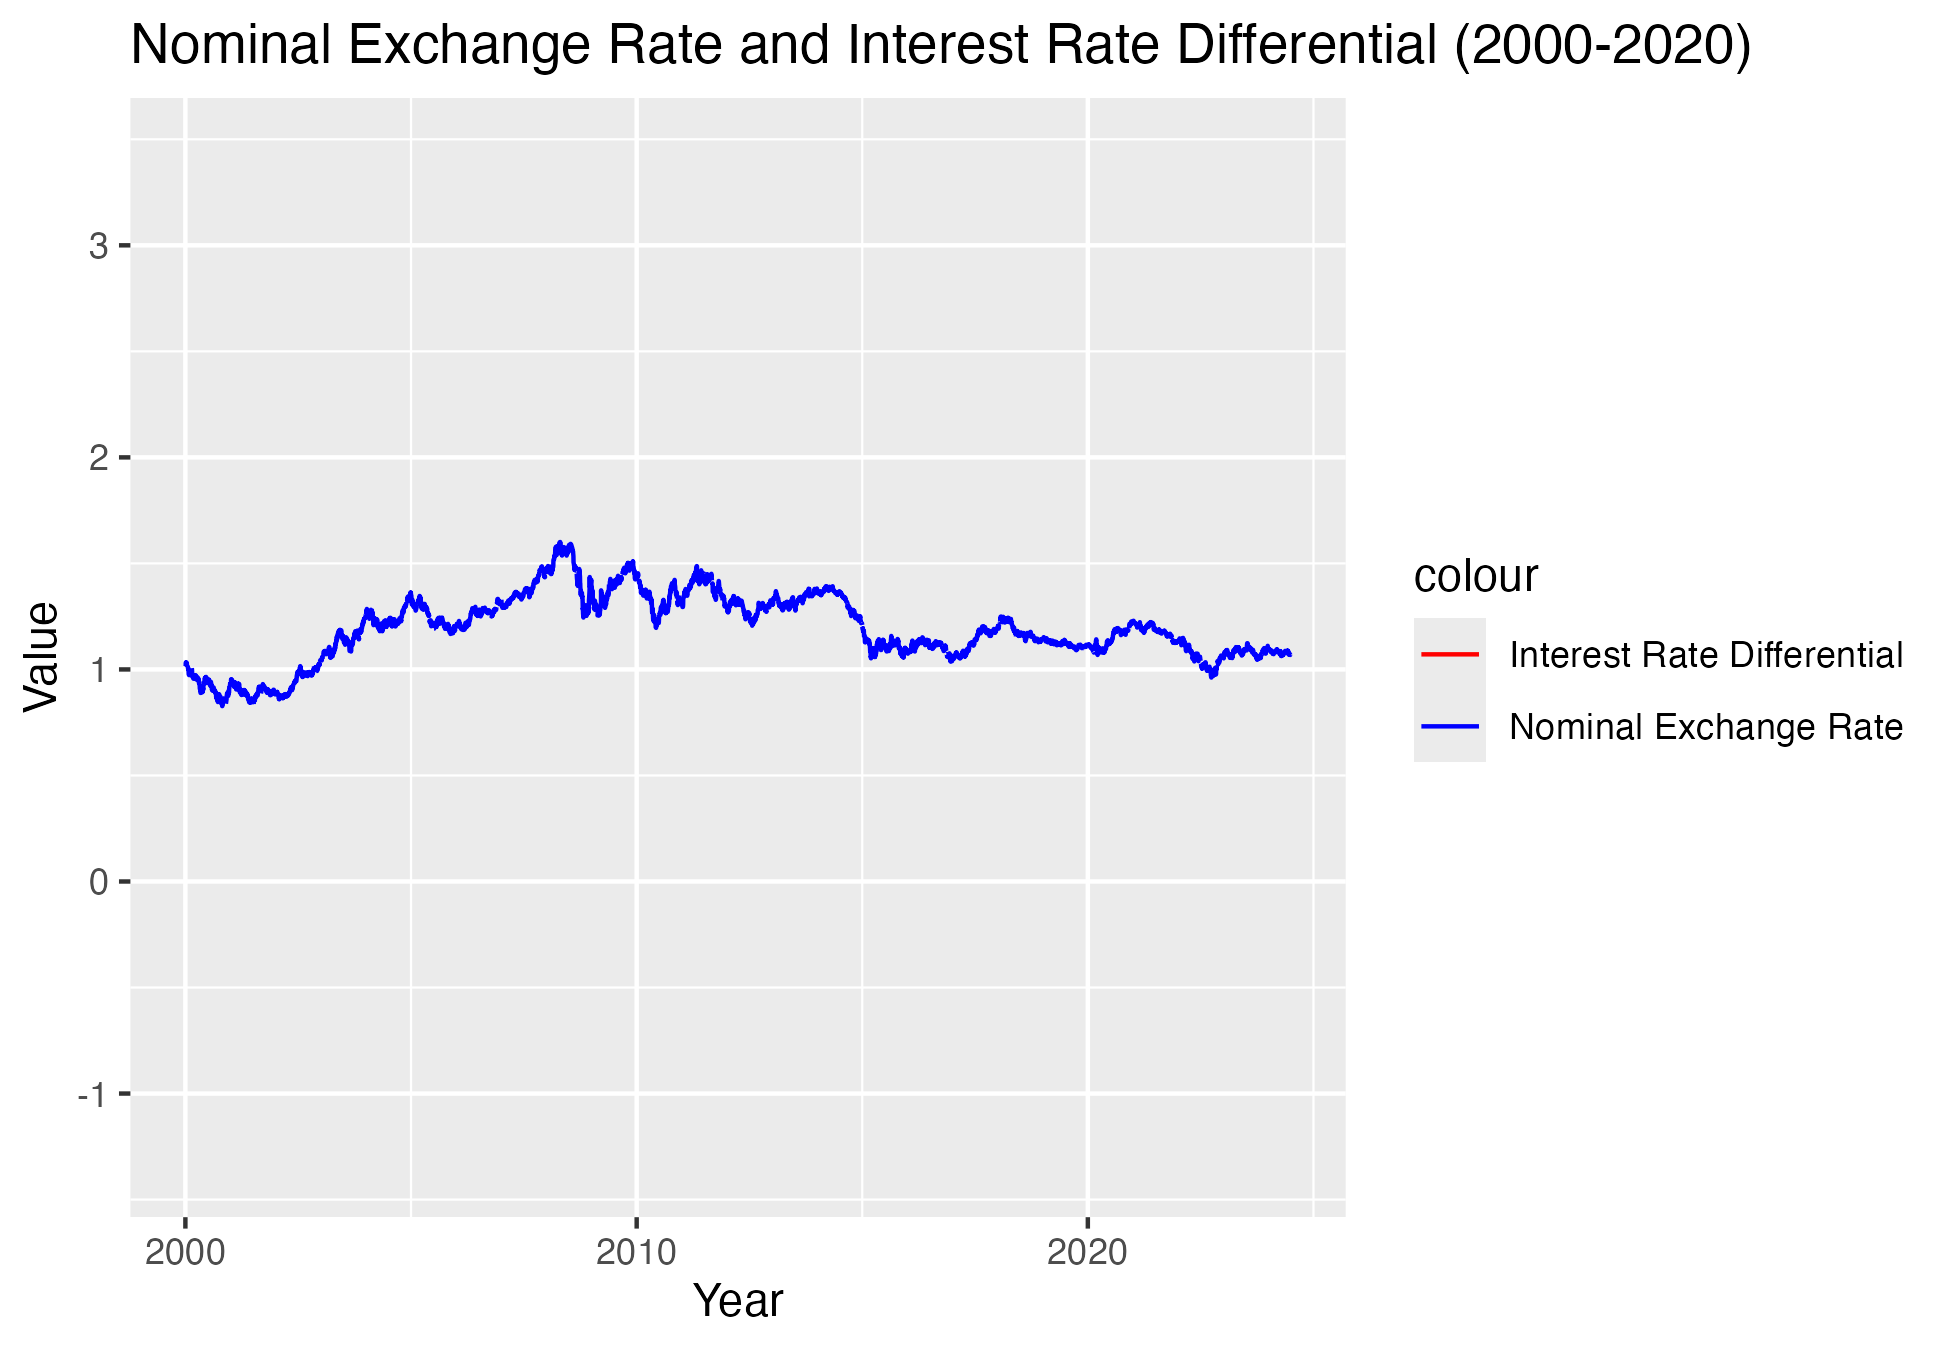
\includegraphics[width=0.9\textwidth]{/Users/cancel/Personal/Coursework/Econ425/VA1/R/Nominal_Exchange_Rate_and_Interest_Rate_Differential.png}
    \caption{Nominal Exchange Rate and Interest Rate Differential}
\end{figure}

\hrulefill

\section{Market Assumptions Beyond Perfect Competition}

\textbf{Question 4:} The perfect competition assumption is at odds with the real world. How can we incorporate a more realistic assumption into our understanding of the macroeconomy?

\textbf{4.1 Perfect Competition Assumption:} In a perfectly competitive market, many small firms sell identical products, there are no barriers to entry or exit, and all firms and consumers have perfect information. Firms are price takers, meaning they cannot influence the market price.

\textbf{4.2 More Realistic Assumptions:} To incorporate more realistic assumptions, we can consider:

\begin{itemize}
    \item \textbf{Monopolistic Competition:} Many firms sell products that are similar but not identical. Each firm has some degree of market power to set prices. Examples include the market for restaurants or clothing brands.
    \item \textbf{Oligopoly:} A few large firms dominate the market. These firms are interdependent, meaning the actions of one firm affect the others. Examples include the automobile and airline industries.
    \item \textbf{Market Imperfections:} Real-world markets have various imperfections such as price stickiness (prices do not adjust immediately to changes in supply and demand), information asymmetries (buyers and sellers do not have the same information), and varying degrees of market power (some firms can influence prices).
\end{itemize}

\hrulefill

\section{Price Rigidity and Market Power}

\textbf{Question 5:} Empirically, prices are not (fully) flexible. Does this mean firms have market power? What does this imply for the macroeconomy?

\textbf{5.1 Price Rigidity:} Price rigidity refers to the situation where prices do not adjust immediately to changes in supply and demand. Prices may be sticky due to menu costs (the costs of changing prices), contracts, or strategic reasons.

\textbf{5.2 Market Power:} Firms with market power can set prices above marginal cost, leading to price rigidity. They do not have to adjust prices frequently because they are not price takers.

\textbf{5.3 Implications for the Macroeconomy:} Price rigidity can lead to prolonged periods of disequilibrium, where supply and demand are not balanced. This can result in unemployment (when prices are too high) or shortages (when prices are too low). It can slow down the economy’s response to shocks, making it harder for monetary and fiscal policies to stabilize the economy.

\textbf{Graph: Consumer Price Index:} 

To illustrate price rigidity, we plot the Consumer Price Index (CPI) over time. The CPI is a measure of the average change in prices paid by consumers for goods and services. A steady rise in the CPI indicates persistent inflation, while fluctuations may suggest price rigidity or volatility.

\begin{figure}[h!]
    \centering
    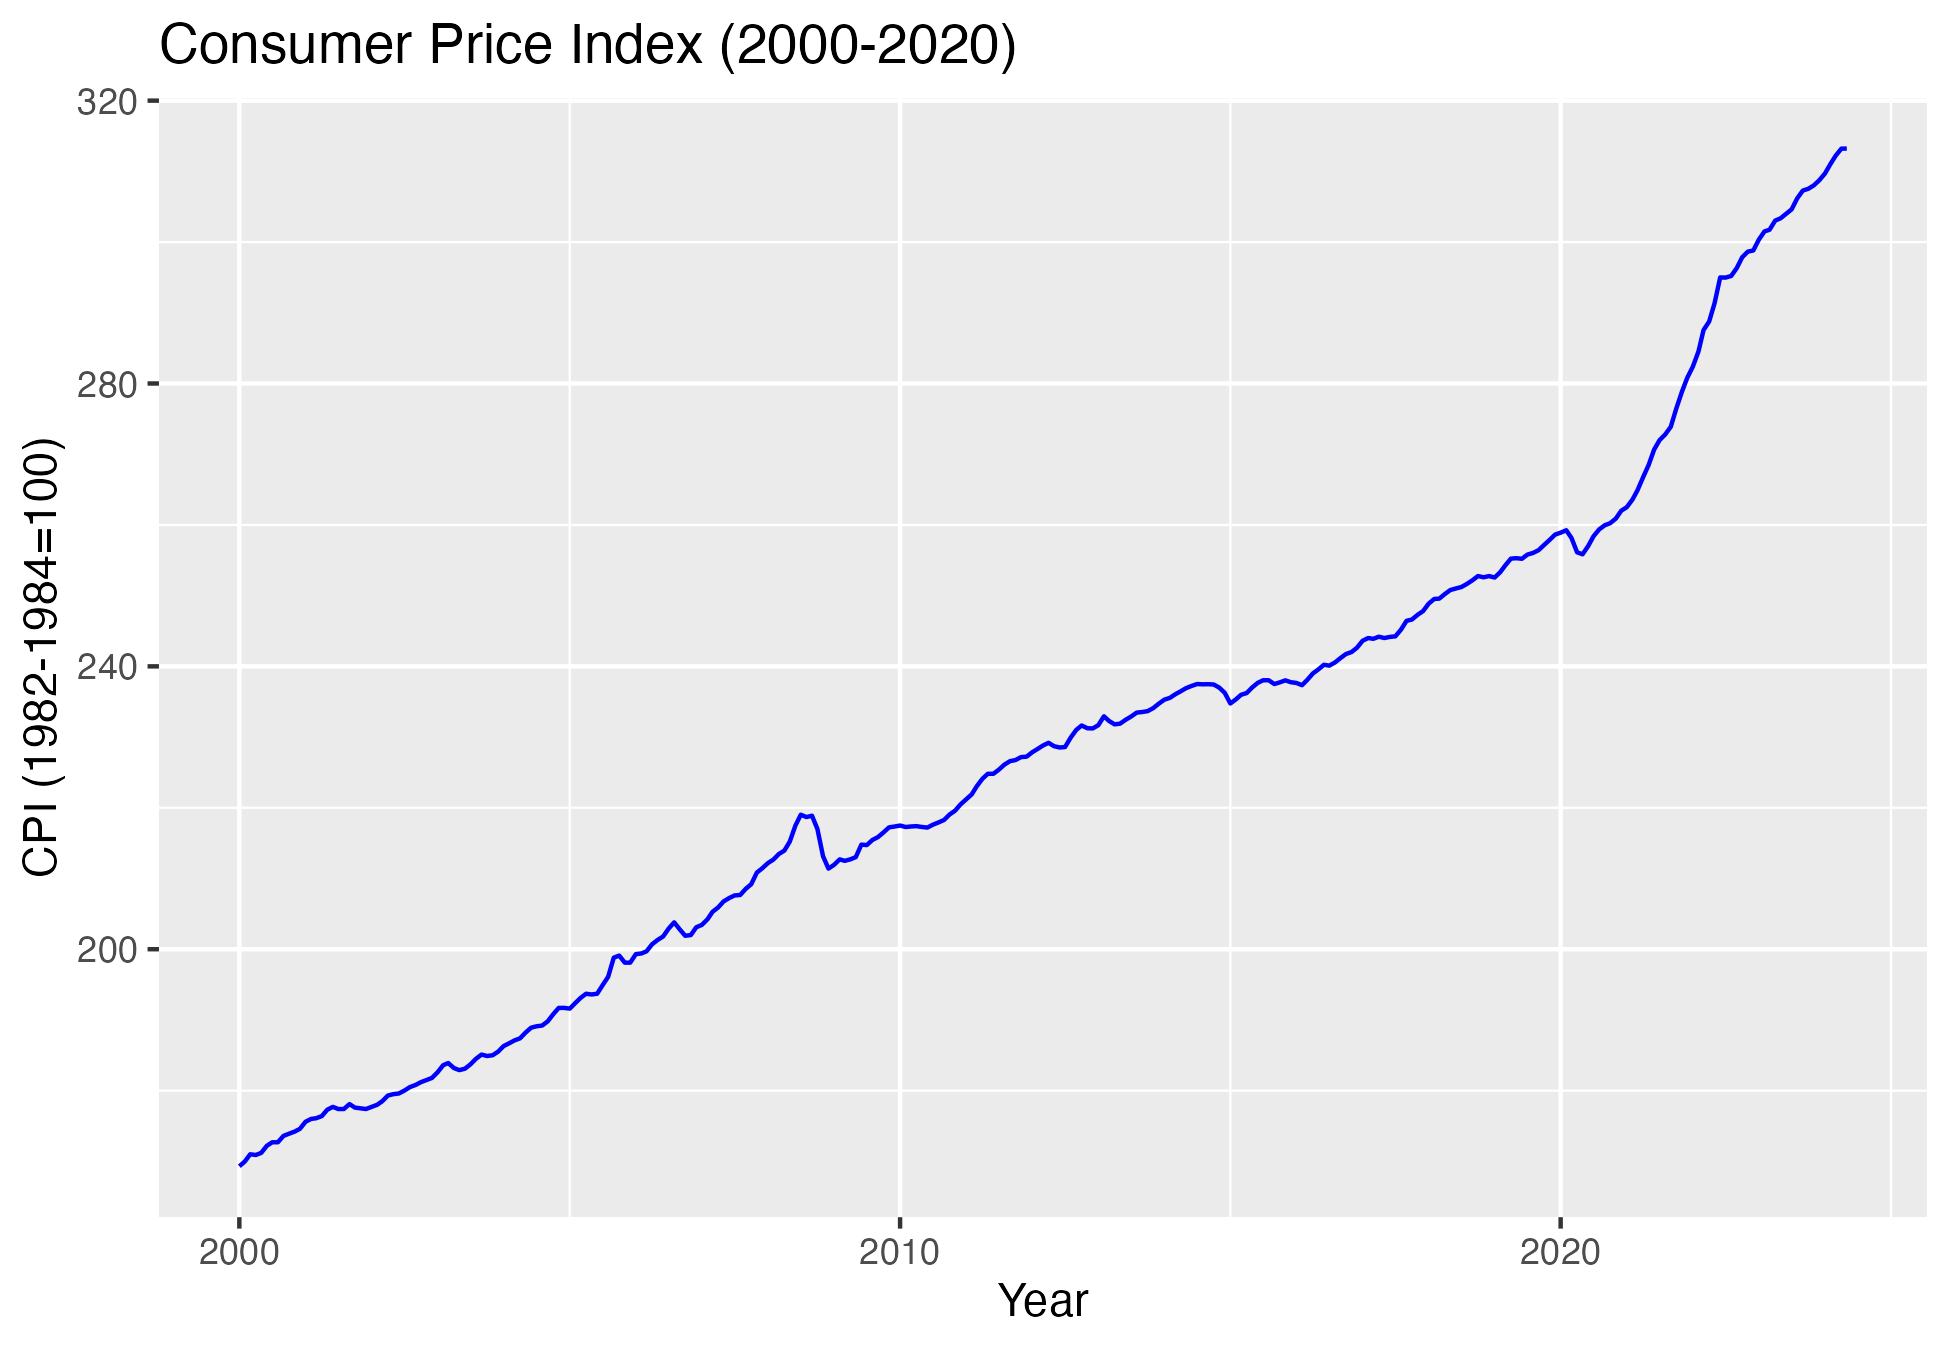
\includegraphics[width=0.9\textwidth]{/Users/cancel/Personal/Coursework/Econ425/VA1/R/Consumer_Price_Index.png}
    \caption{Consumer Price Index}
\end{figure}

\hrulefill

\section{Natural Level of Output and Output Gap}

\textbf{Question 6:} What is the 'natural level of output' and what is the ``output gap''? Is there any relationship between them? Can we observe or estimate any of them in reality? Are these things related to the Natural Rate Hypothesis?

\textbf{6.1 Natural Level of Output:} The natural level of output, also known as potential output, is the level of production an economy can achieve when operating at full capacity, with full employment and optimal use of resources. It is determined by factors such as technology, labor, and capital.

\textbf{6.2 Output Gap:} The output gap is the difference between actual output and the natural level of output. It can be positive or negative:

\begin{itemize}
    \item \textbf{Positive Output Gap:} When actual output exceeds potential output, it can lead to inflationary pressures as demand outstrips supply.
    \item \textbf{Negative Output Gap:} When actual output is below potential output, it can lead to unemployment and underused resources, indicating that the economy is not operating at full capacity.
\end{itemize}

\textbf{6.3 Natural Rate Hypothesis:} The natural rate hypothesis proposes that the economy tends toward the natural rate of unemployment and the natural level of output in the long run, regardless of short-term fluctuations. It suggests that there is a level of unemployment that is consistent with a stable inflation rate.

\textbf{Graph: Actual vs. Potential Output:} 

To visualize the concept of the output gap, we plot actual GDP against potential GDP. The blue line represents actual GDP, while the red line represents potential GDP. The difference between these two lines indicates the output gap, highlighting periods of economic expansion and contraction.

\begin{figure}[h!]
    \centering
    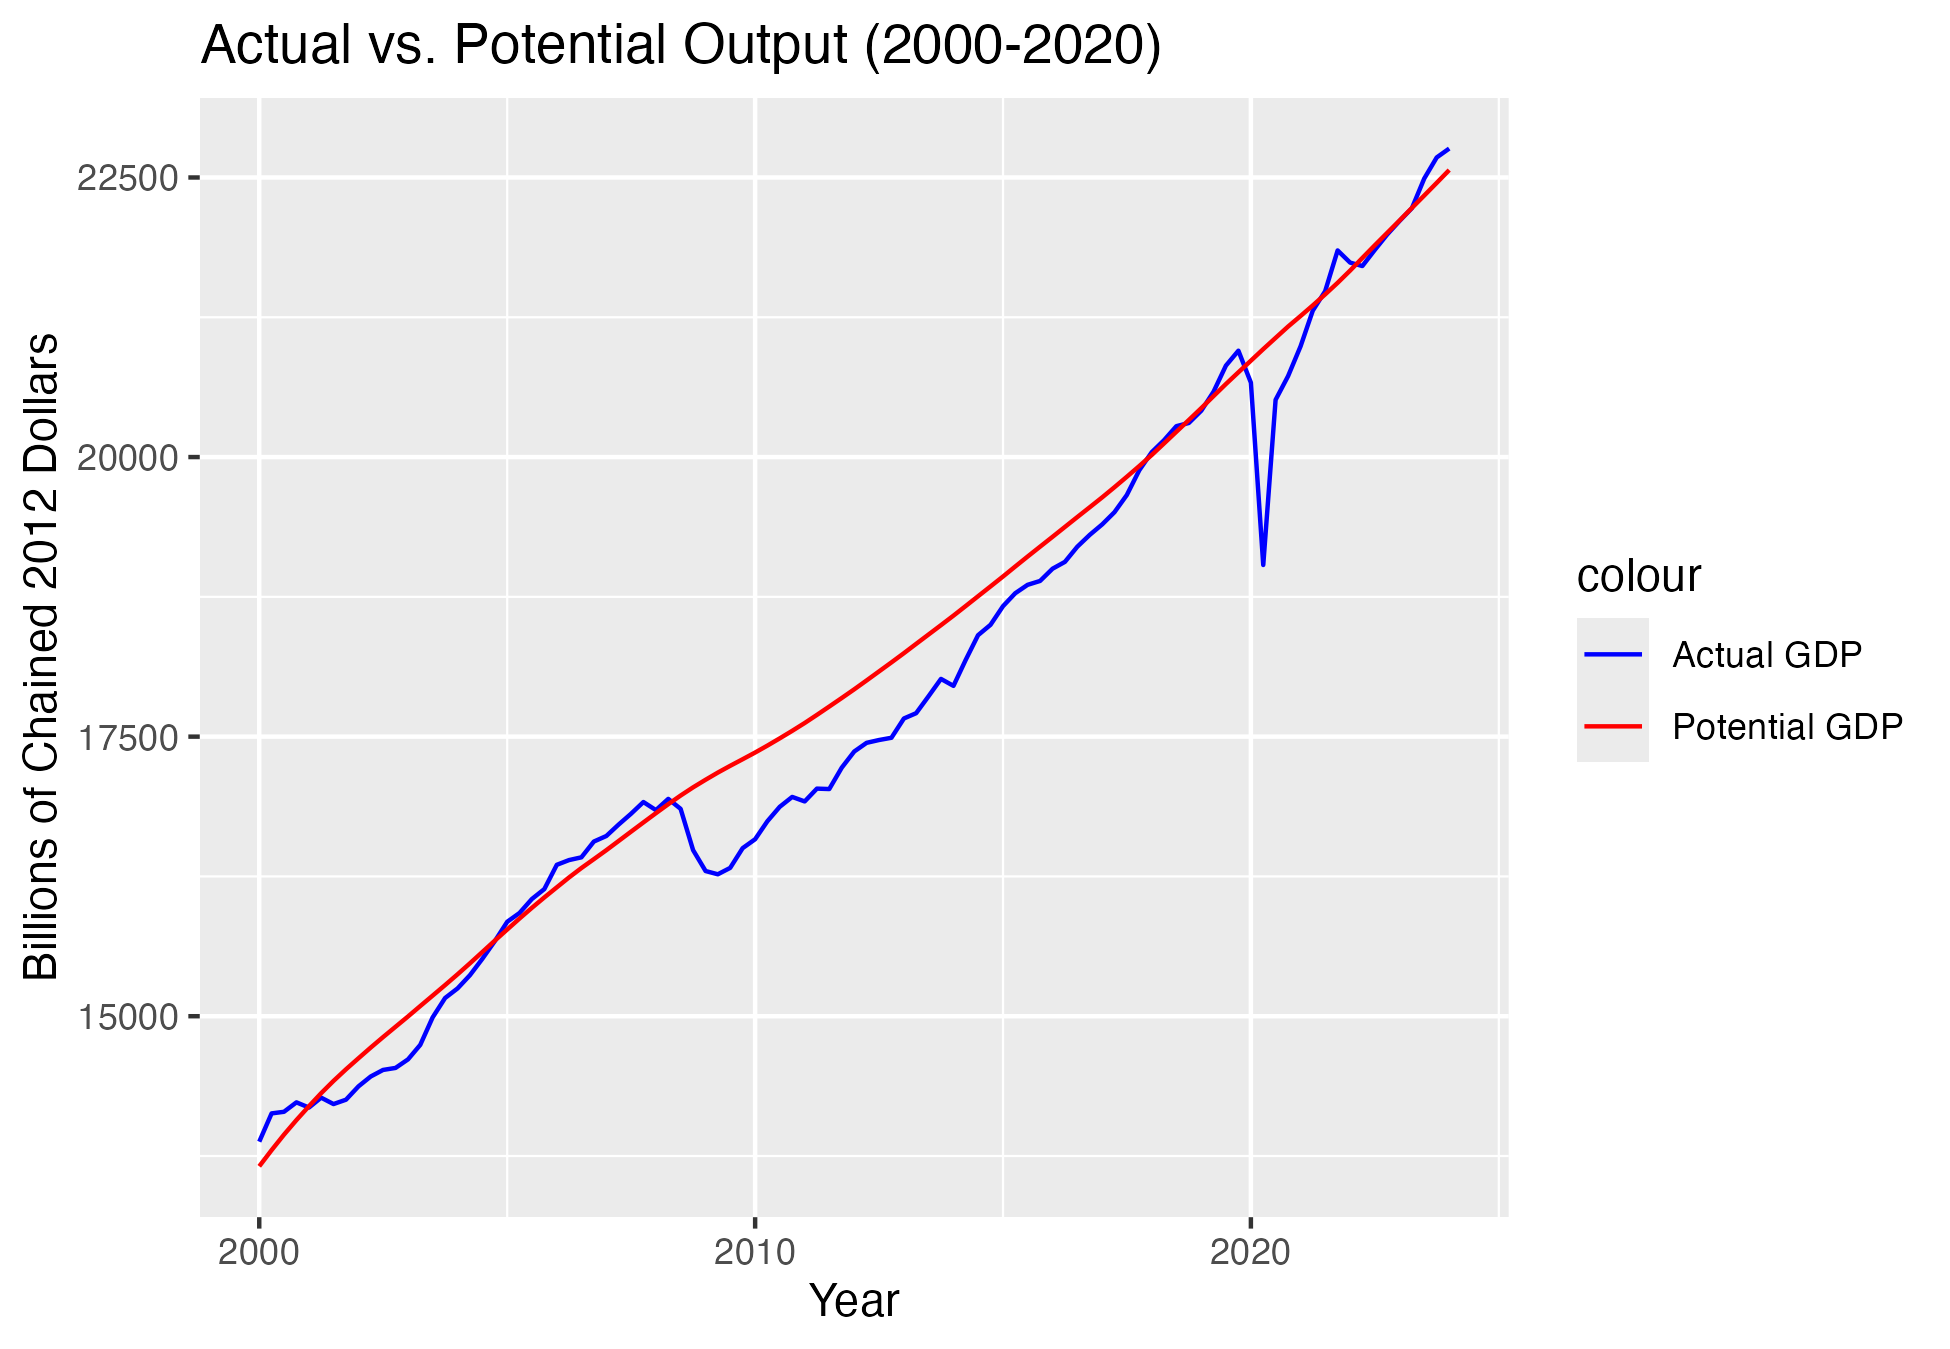
\includegraphics[width=0.9\textwidth]{/Users/cancel/Personal/Coursework/Econ425/VA1/R/Actual_vs_Potential_Output.png}
    \caption{Actual vs. Potential Output}
\end{figure}

\hrulefill

\section{Phillips Curve}

\textbf{Question 7:} What is the Phillips Curve and why is it called that way?

\textbf{7.1 Phillips Curve:} The Phillips Curve represents the inverse relationship between inflation and unemployment in the short run. It suggests that lower unemployment leads to higher inflation and vice versa. The Phillips Curve is named after economist A.W. Phillips, who first identified this relationship by analyzing historical data on wage inflation and unemployment in the UK.

\textbf{Graph: Phillips Curve:} 

The Phillips Curve graph plots the relationship between the unemployment rate and the inflation rate. Each point represents a pair of unemployment and inflation rates for a specific period. The red line shows the trend, indicating the trade-off between inflation and unemployment.

\begin{figure}[h!]
    \centering
    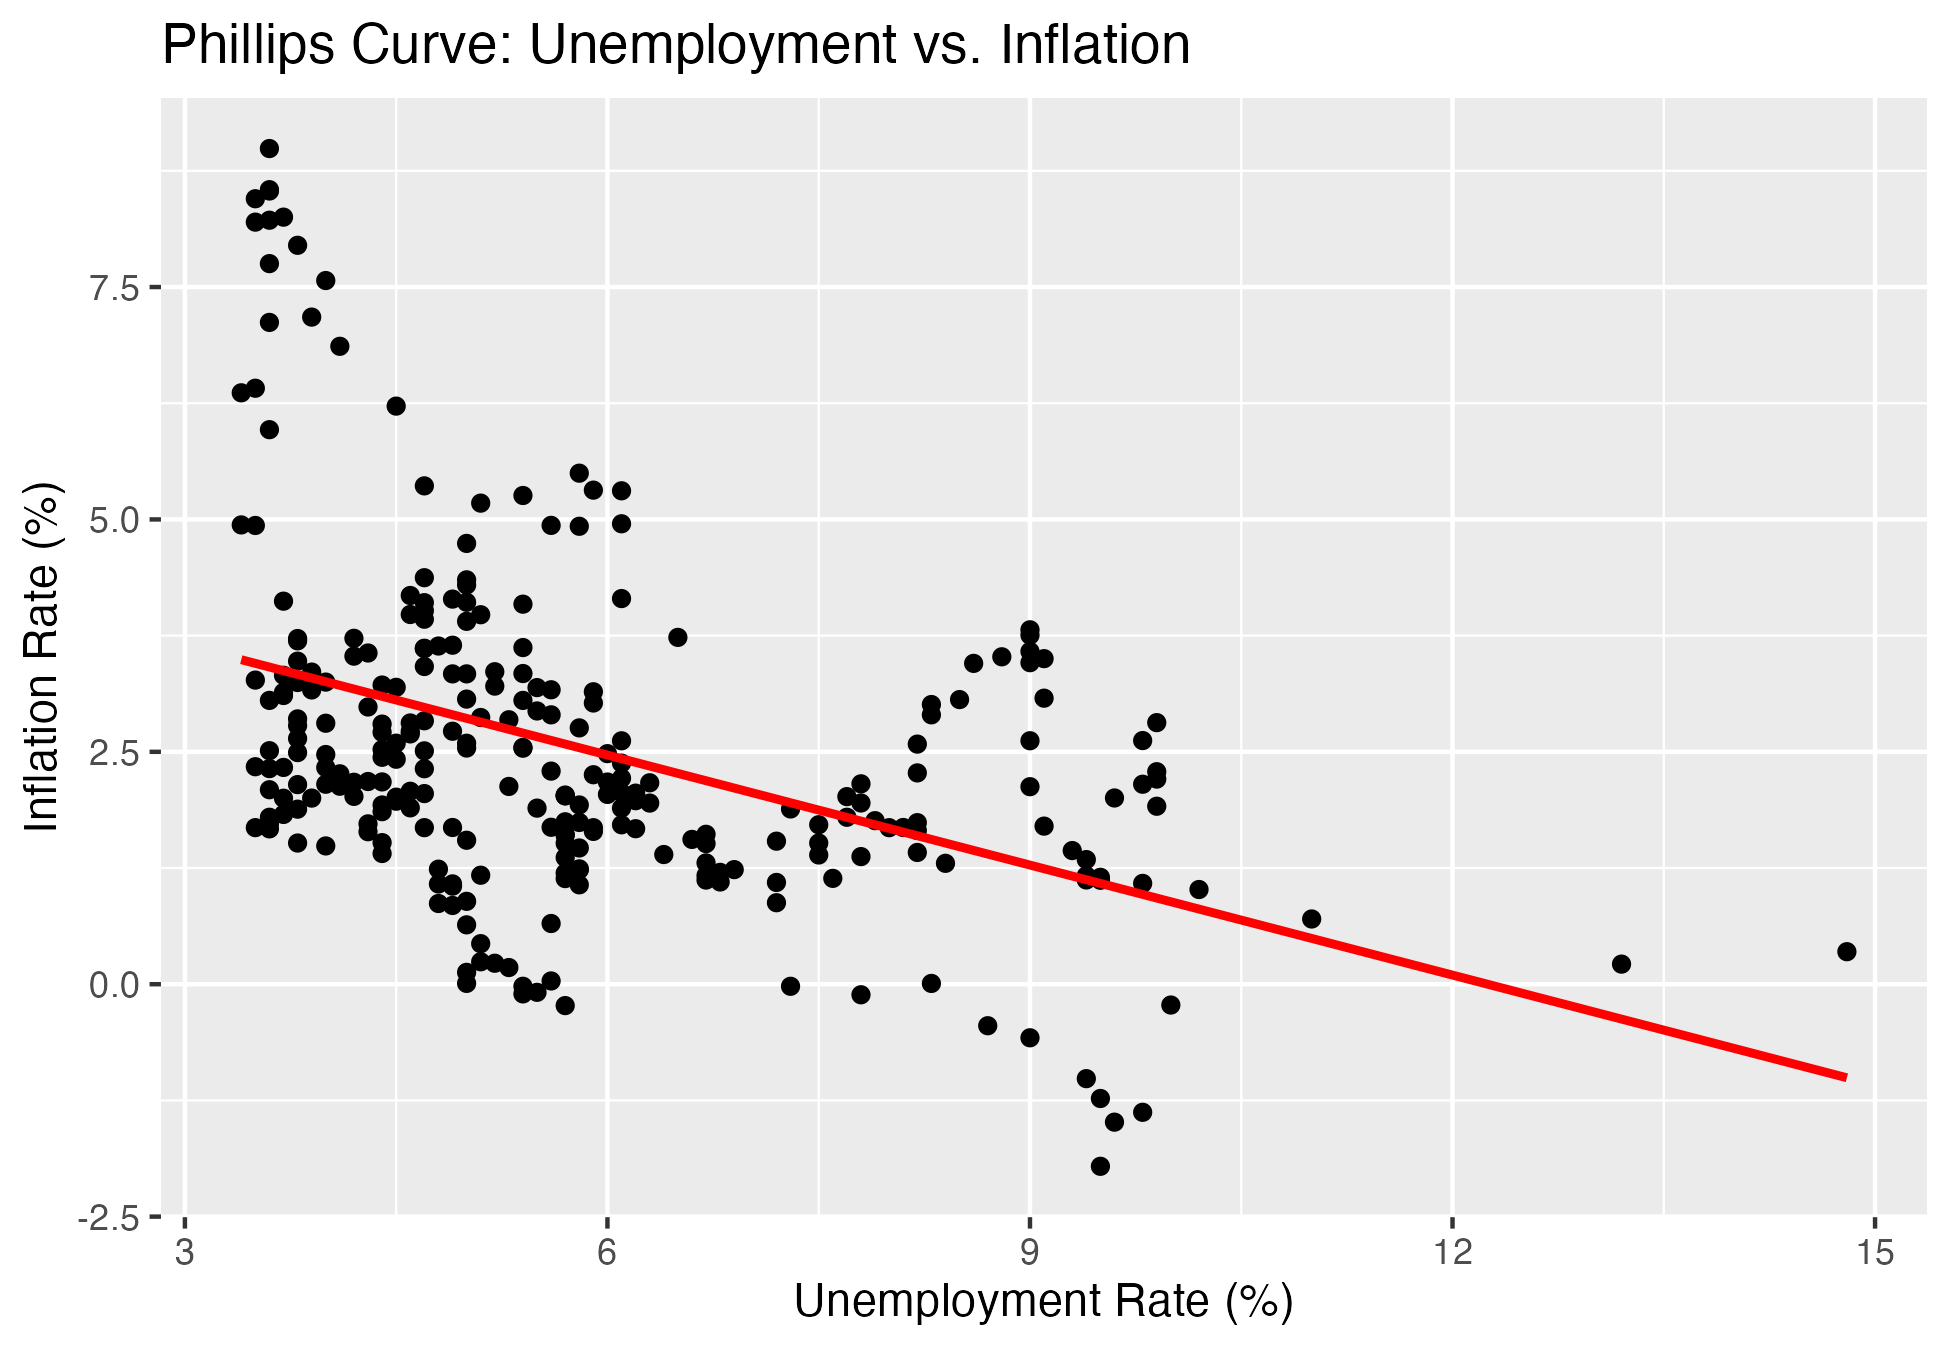
\includegraphics[width=0.9\textwidth]{/Users/cancel/Personal/Coursework/Econ425/VA1/R/Phillips_Curve.png}
    \caption{Phillips Curve}
\end{figure}

\hrulefill

\section{Shocks in Macroeconomics}

\textbf{Question 8:} Explain what is a shock and in what context they appear in macroeconomics. How can we think of a shock in theory versus in reality? Provide examples.

\textbf{8.1 Shock:} A shock is an unexpected event that affects the economy. Shocks can be positive or negative and can originate from various sources.

\textbf{8.2 Types of Shocks:} Shocks can be:

\begin{itemize}
    \item \textbf{Supply Shock:} Affects the supply side of the economy. For example, a sudden increase in oil prices raises production costs and can lead to higher inflation and lower output.
    \item \textbf{Demand Shock:} Affects the demand side of the economy. For example, a sudden increase in consumer confidence can boost spending and increase overall demand.
\end{itemize}

\textbf{8.3 In Theory vs. Reality:} In theory, shocks are often modeled as sudden changes in variables like technology, preferences, or policy. In reality, shocks can be events like financial crises, natural disasters, or unexpected policy changes.

\textbf{Graph: Impact of Supply Shocks on GDP:} 

To illustrate the impact of supply shocks, we plot GDP with a simulated supply shock. The blue line represents normal GDP, while the red line shows GDP under a supply shock. This graph helps visualize how sudden changes in supply can affect overall economic output.

\begin{figure}[h!]
    \centering
    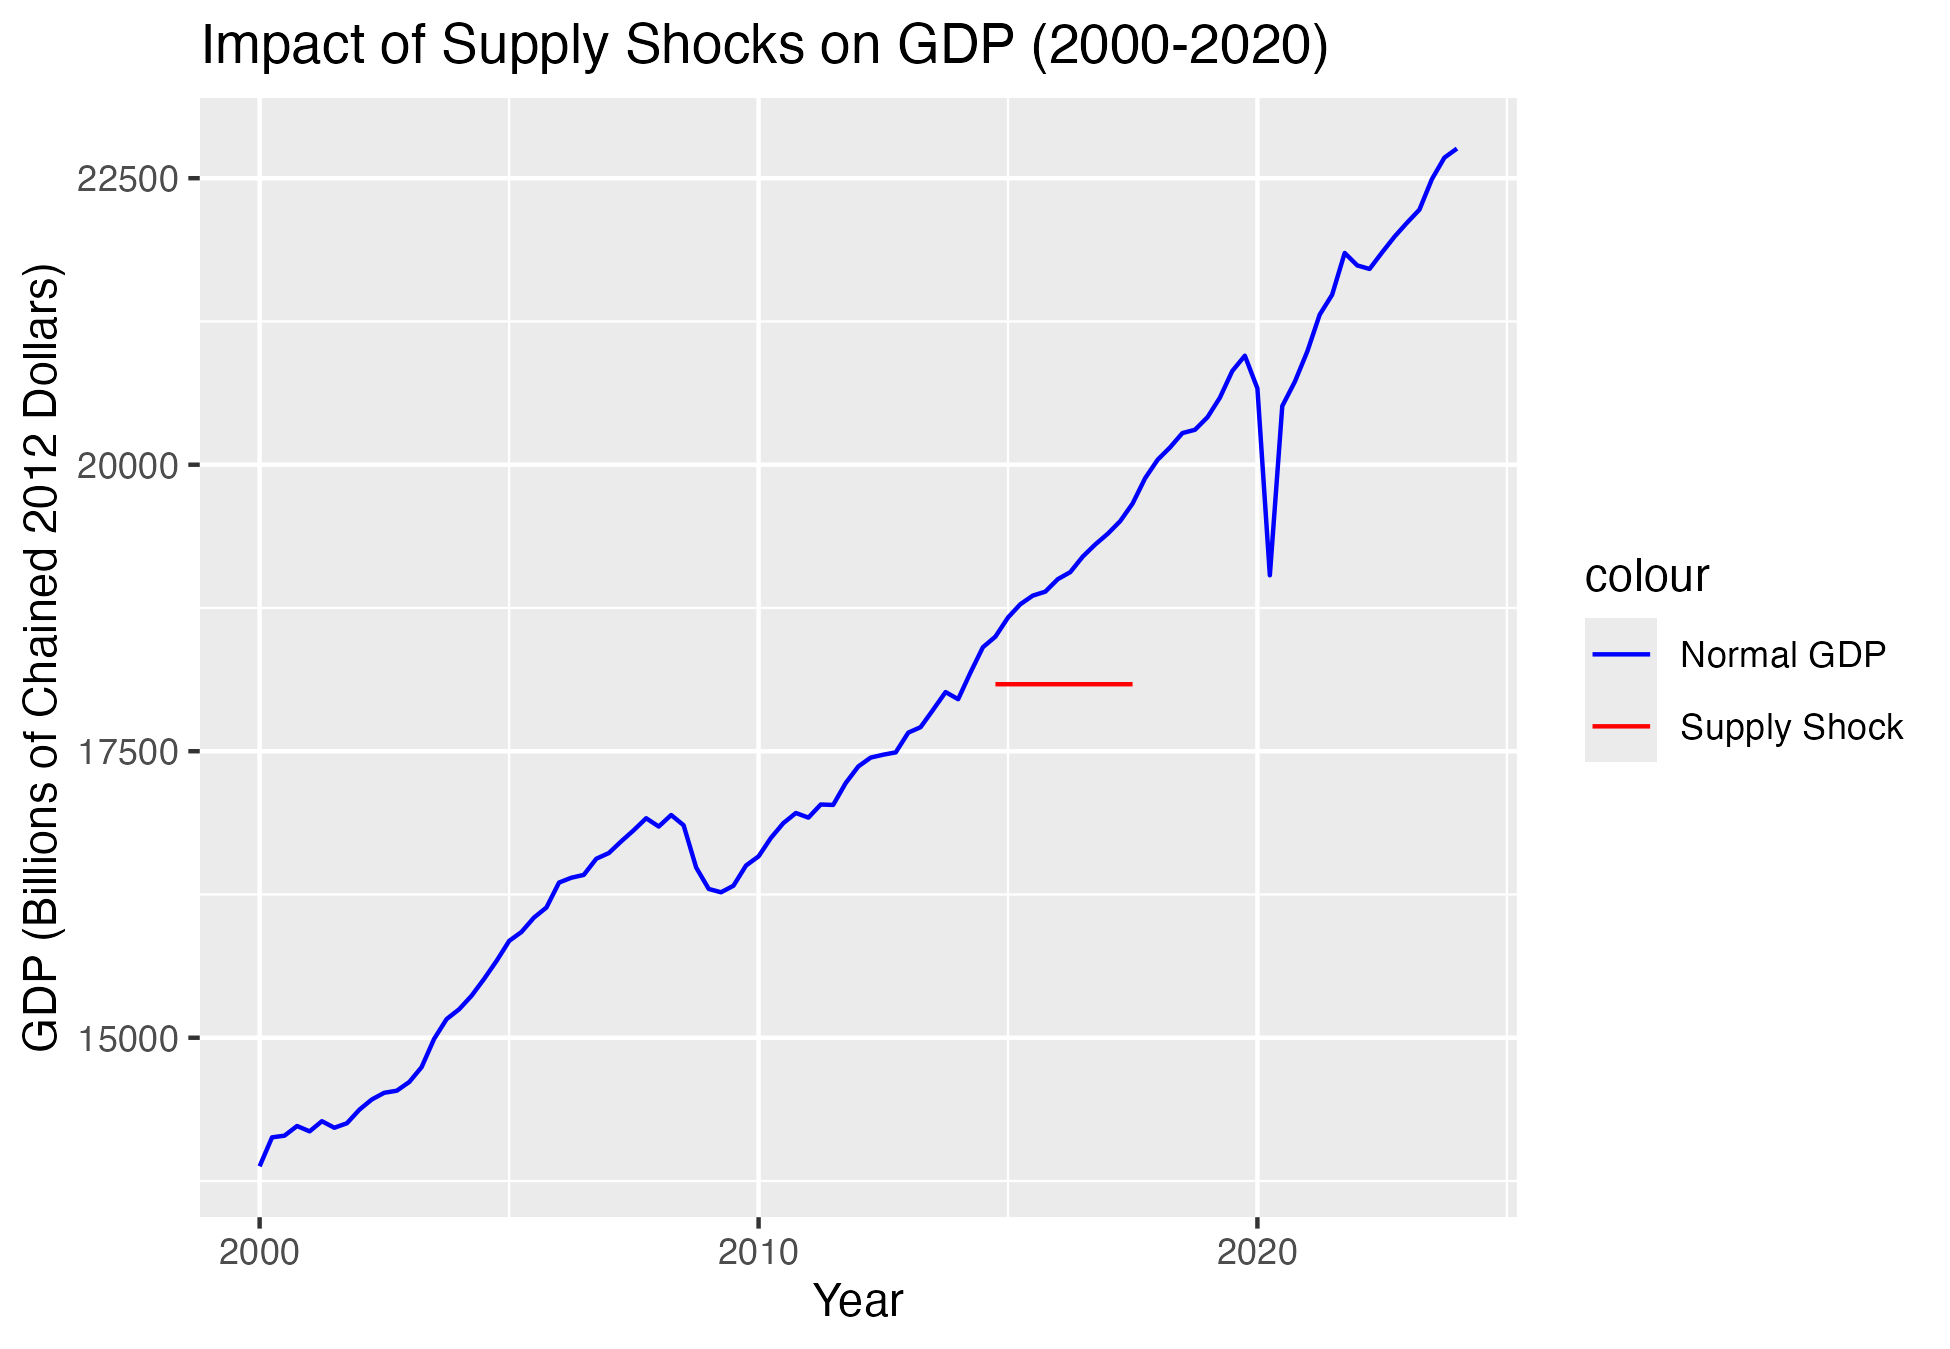
\includegraphics[width=0.9\textwidth]{/Users/cancel/Personal/Coursework/Econ425/VA1/R/Impact_of_Supply_Shocks_on_GDP.png}
    \caption{Impact of Supply Shocks on GDP}
\end{figure}

\hrulefill

\section{Monetary Policy Shock as an AD Shock}

\textbf{Question 9:} Explain how and why a monetary policy shock can be seen as a form of AD shock.

\textbf{9.1 Monetary Policy Shock:} A monetary policy shock is an unexpected change in monetary policy, such as a sudden increase or decrease in interest rates or changes in money supply.

\textbf{9.2 Aggregate Demand (AD) Shock:} A monetary policy shock can be seen as an AD shock because it directly affects aggregate demand. For example:

\begin{itemize}
    \item \textbf{Expansionary Monetary Policy:} Lower interest rates or increased money supply can boost consumption and investment, shifting the AD curve to the right.
    \item \textbf{Contractionary Monetary Policy:} Higher interest rates or reduced money supply can reduce consumption and investment, shifting the AD curve to the left.
\end{itemize}

\textbf{Graph: Impact of Monetary Policy on GDP:} 

This graph shows the impact of monetary policy on GDP. The blue line represents GDP, while the red dashed line shows the federal funds rate, which is a key indicator of monetary policy. This visual helps understand how changes in monetary policy affect economic output.

\begin{figure}[h!]
    \centering
    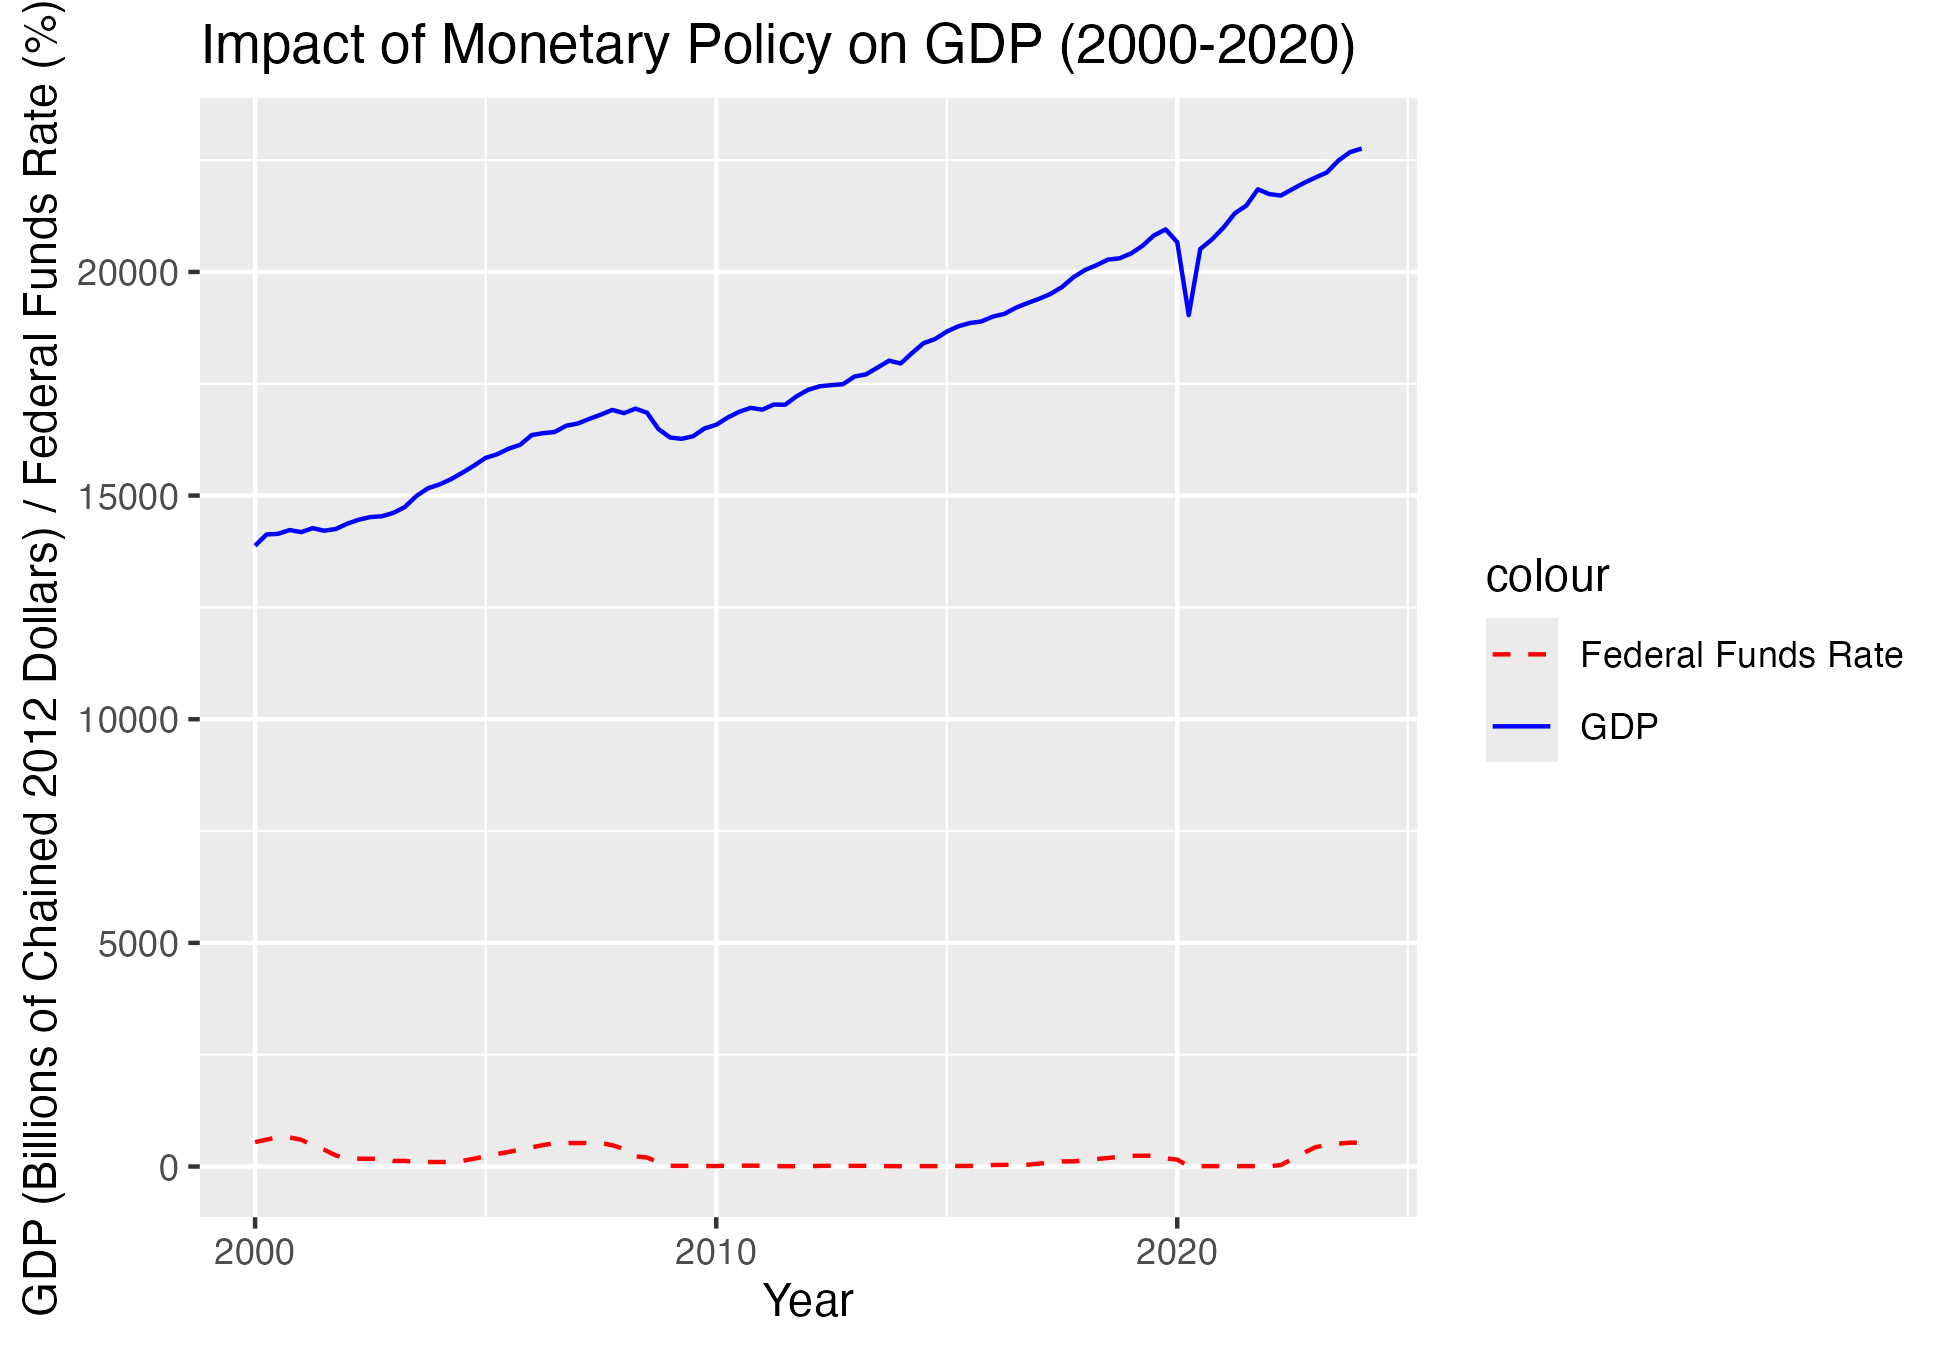
\includegraphics[width=0.9\textwidth]{/Users/cancel/Personal/Coursework/Econ425/VA1/R/Impact_of_Monetary_Policy_on_GDP.png}
    \caption{Impact of Monetary Policy on GDP}
\end{figure}

\hrulefill

\section{Productivity Shock Mechanism}

\textbf{Question 10:} Explain the mechanism through which a productivity shock affects the economy.

\textbf{10.1 Productivity Shock:} A productivity shock is a sudden change in the productivity of labor or capital. It can be positive (improvement in technology) or negative (natural disaster).

\textbf{10.2 Mechanism:} A productivity shock affects the economy as follows:

\begin{itemize}
    \item \textbf{Positive Productivity Shock:} Increases output, lowers prices, and can lead to higher wages and employment. It boosts economic growth and improves living standards.
    \item \textbf{Negative Productivity Shock:} Reduces output, raises prices, and can lead to lower wages and employment. It can slow down economic growth and reduce living standards.
\end{itemize}

\textbf{Graph: Impact of Productivity Shocks on GDP:} 

To illustrate the impact of productivity shocks, we plot GDP with a simulated positive productivity shock. The blue line represents normal GDP, while the green line shows GDP under a positive productivity shock. This graph demonstrates how improvements in productivity can enhance economic output.

\begin{figure}[h!]
    \centering
    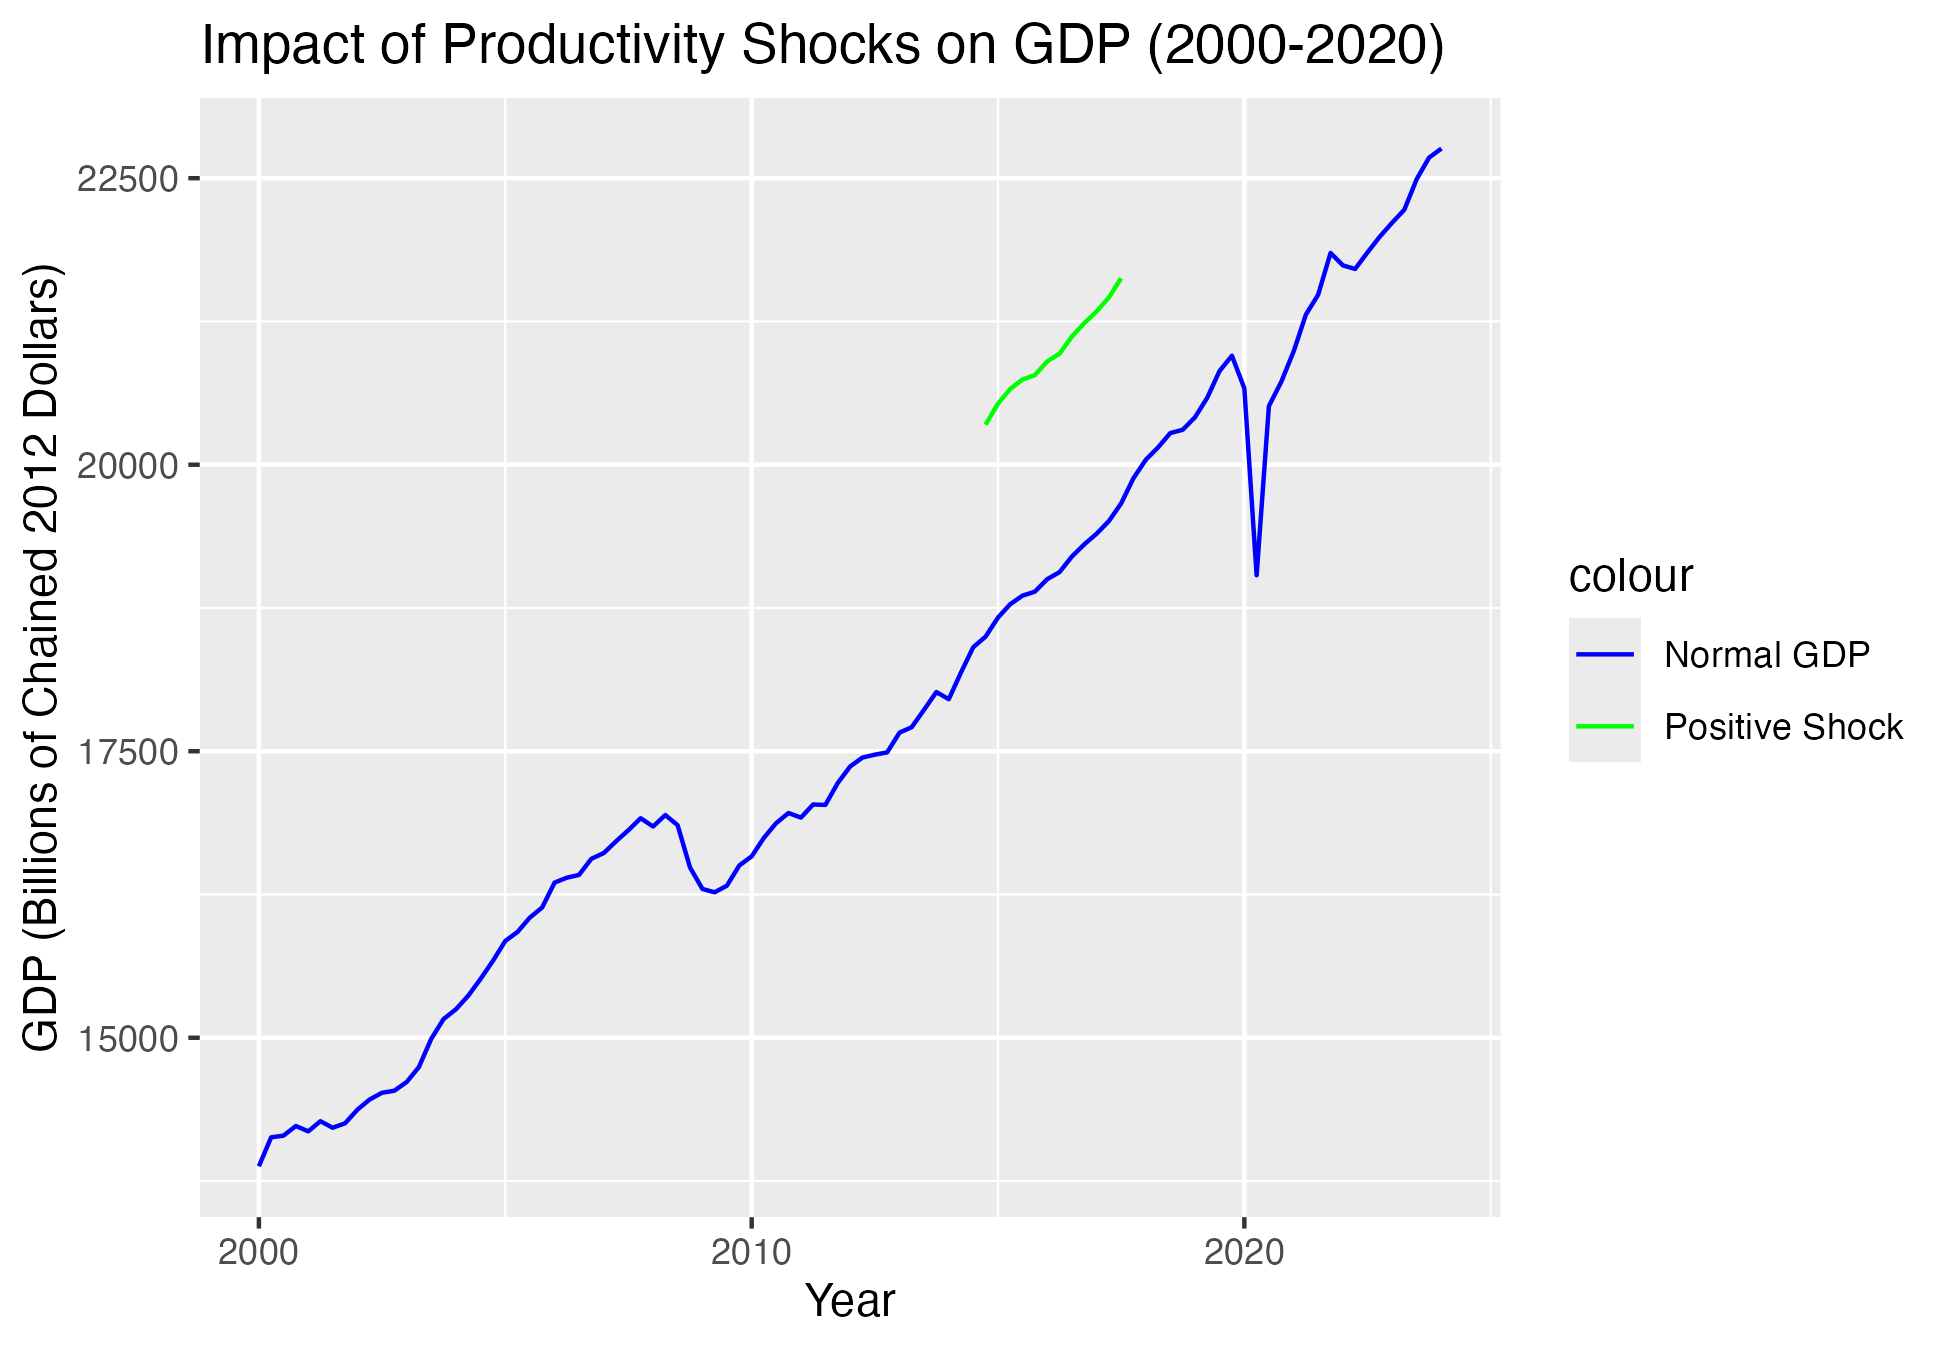
\includegraphics[width=0.9\textwidth]{/Users/cancel/Personal/Coursework/Econ425/VA1/R/Impact_of_Productivity_Shocks_on_GDP.png}
    \caption{Impact of Productivity Shocks on GDP}
\end{figure}

\hrulefill

\section{Business Cycles}

\textbf{Question 11:} What are business cycles and why should we care about them if what we want to do is macroeconomic policy?

\textbf{11.1 Business Cycles:} Business cycles refer to the fluctuations in economic activity characterized by periods of expansion and contraction. These cycles consist of four phases:

\begin{itemize}
    \item \textbf{Expansion:} Increasing economic activity, rising GDP, and falling unemployment.
    \item \textbf{Peak:} The highest point of economic activity before a downturn.
    \item \textbf{Contraction:} Decreasing economic activity, falling GDP, and rising unemployment.
    \item \textbf{Trough:} The lowest point of economic activity before a recovery begins.
\end{itemize}

\textbf{11.2 Importance for Macroeconomic Policy:} Understanding business cycles is crucial for designing effective macroeconomic policies. Policymakers aim to smooth out these cycles to achieve stable economic growth, low unemployment, and stable inflation.

\textbf{Graph: Business Cycles:} 

This graph illustrates business cycles by plotting GDP over time, highlighting periods of expansion (blue), peaks (red), troughs (green), and normal periods. This visual helps us understand the cyclical nature of economic activity.

\begin{figure}[h!]
    \centering
    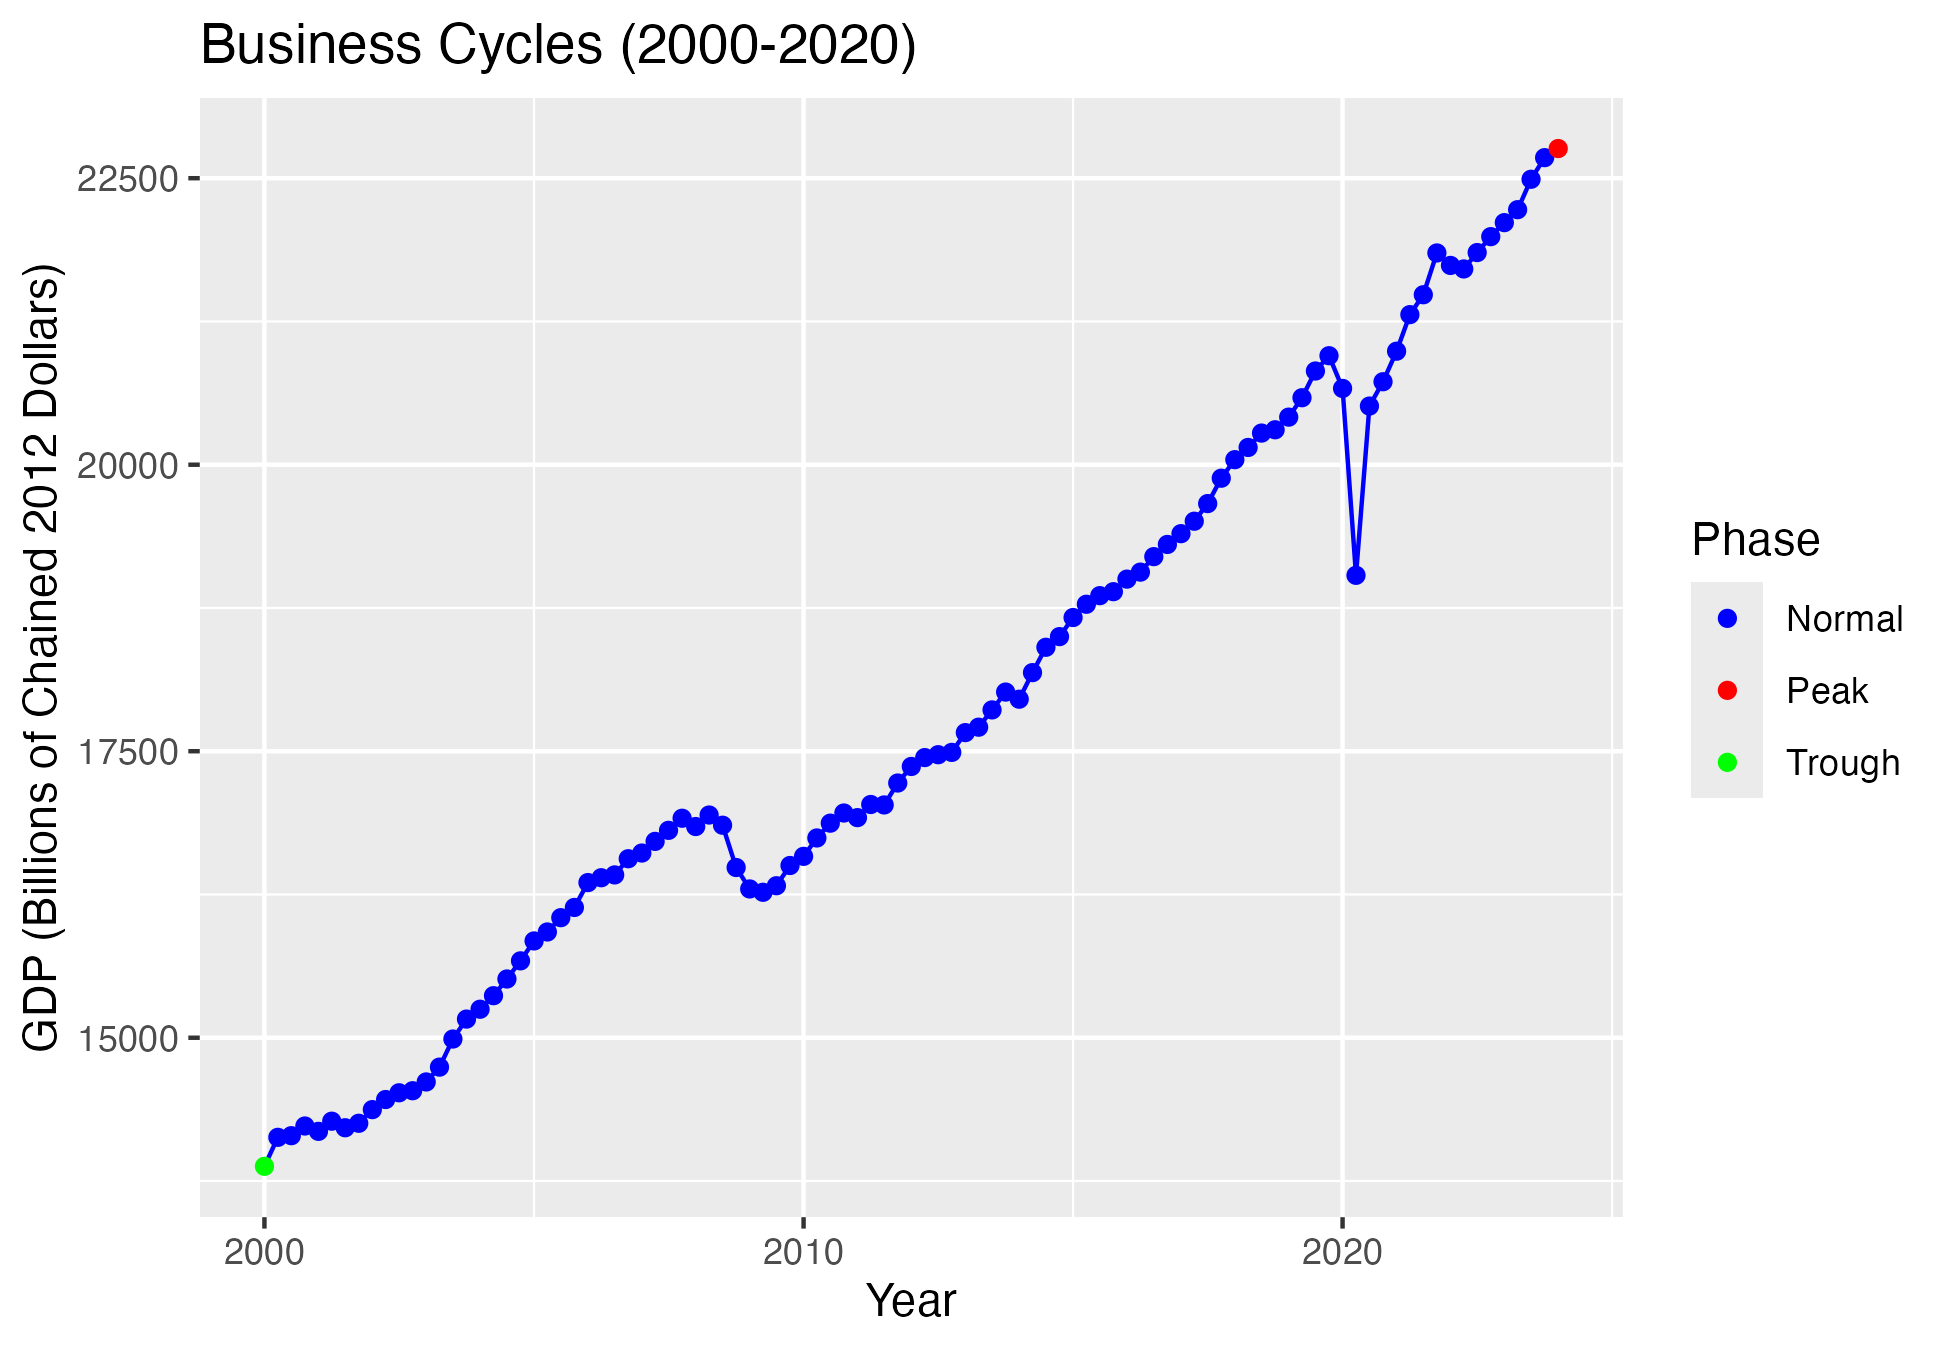
\includegraphics[width=0.9\textwidth]{/Users/cancel/Personal/Coursework/Econ425/VA1/R/Business_Cycles.png}
    \caption{Business Cycles}
\end{figure}

\hrulefill

\section{HP Filter and Cyclical Variables}

\textbf{Question 12:} Speaking of cycles, what is the HP filter and what is its purpose? In addition, when can we say that a variable is procyclical and when is countercyclical? Please provide examples of both.

\textbf{12.1 HP Filter:} The Hodrick-Prescott (HP) filter is a statistical tool used to separate the cyclical component of a time series from its trend component. It helps identify the underlying trend and short-term fluctuations in economic data.

\textbf{12.2 Procyclical vs. Countercyclical:} A variable is procyclical if it moves in the same direction as the overall economy. Examples include investment and consumer spending, which tend to increase during economic expansions and decrease during contractions. A variable is countercyclical if it moves in the opposite direction to the overall economy. Examples include unemployment and government spending on social programs, which tend to increase during economic contractions and decrease during expansions.

\textbf{Graph: HP Filter Applied to GDP:} 

This graph shows the application of the HP filter to GDP. The blue line represents actual GDP, the red line shows the trend component, and the green line indicates the cyclical component. This visual helps us understand the underlying trend and cyclical fluctuations in GDP.

\begin{figure}[h!]
    \centering
    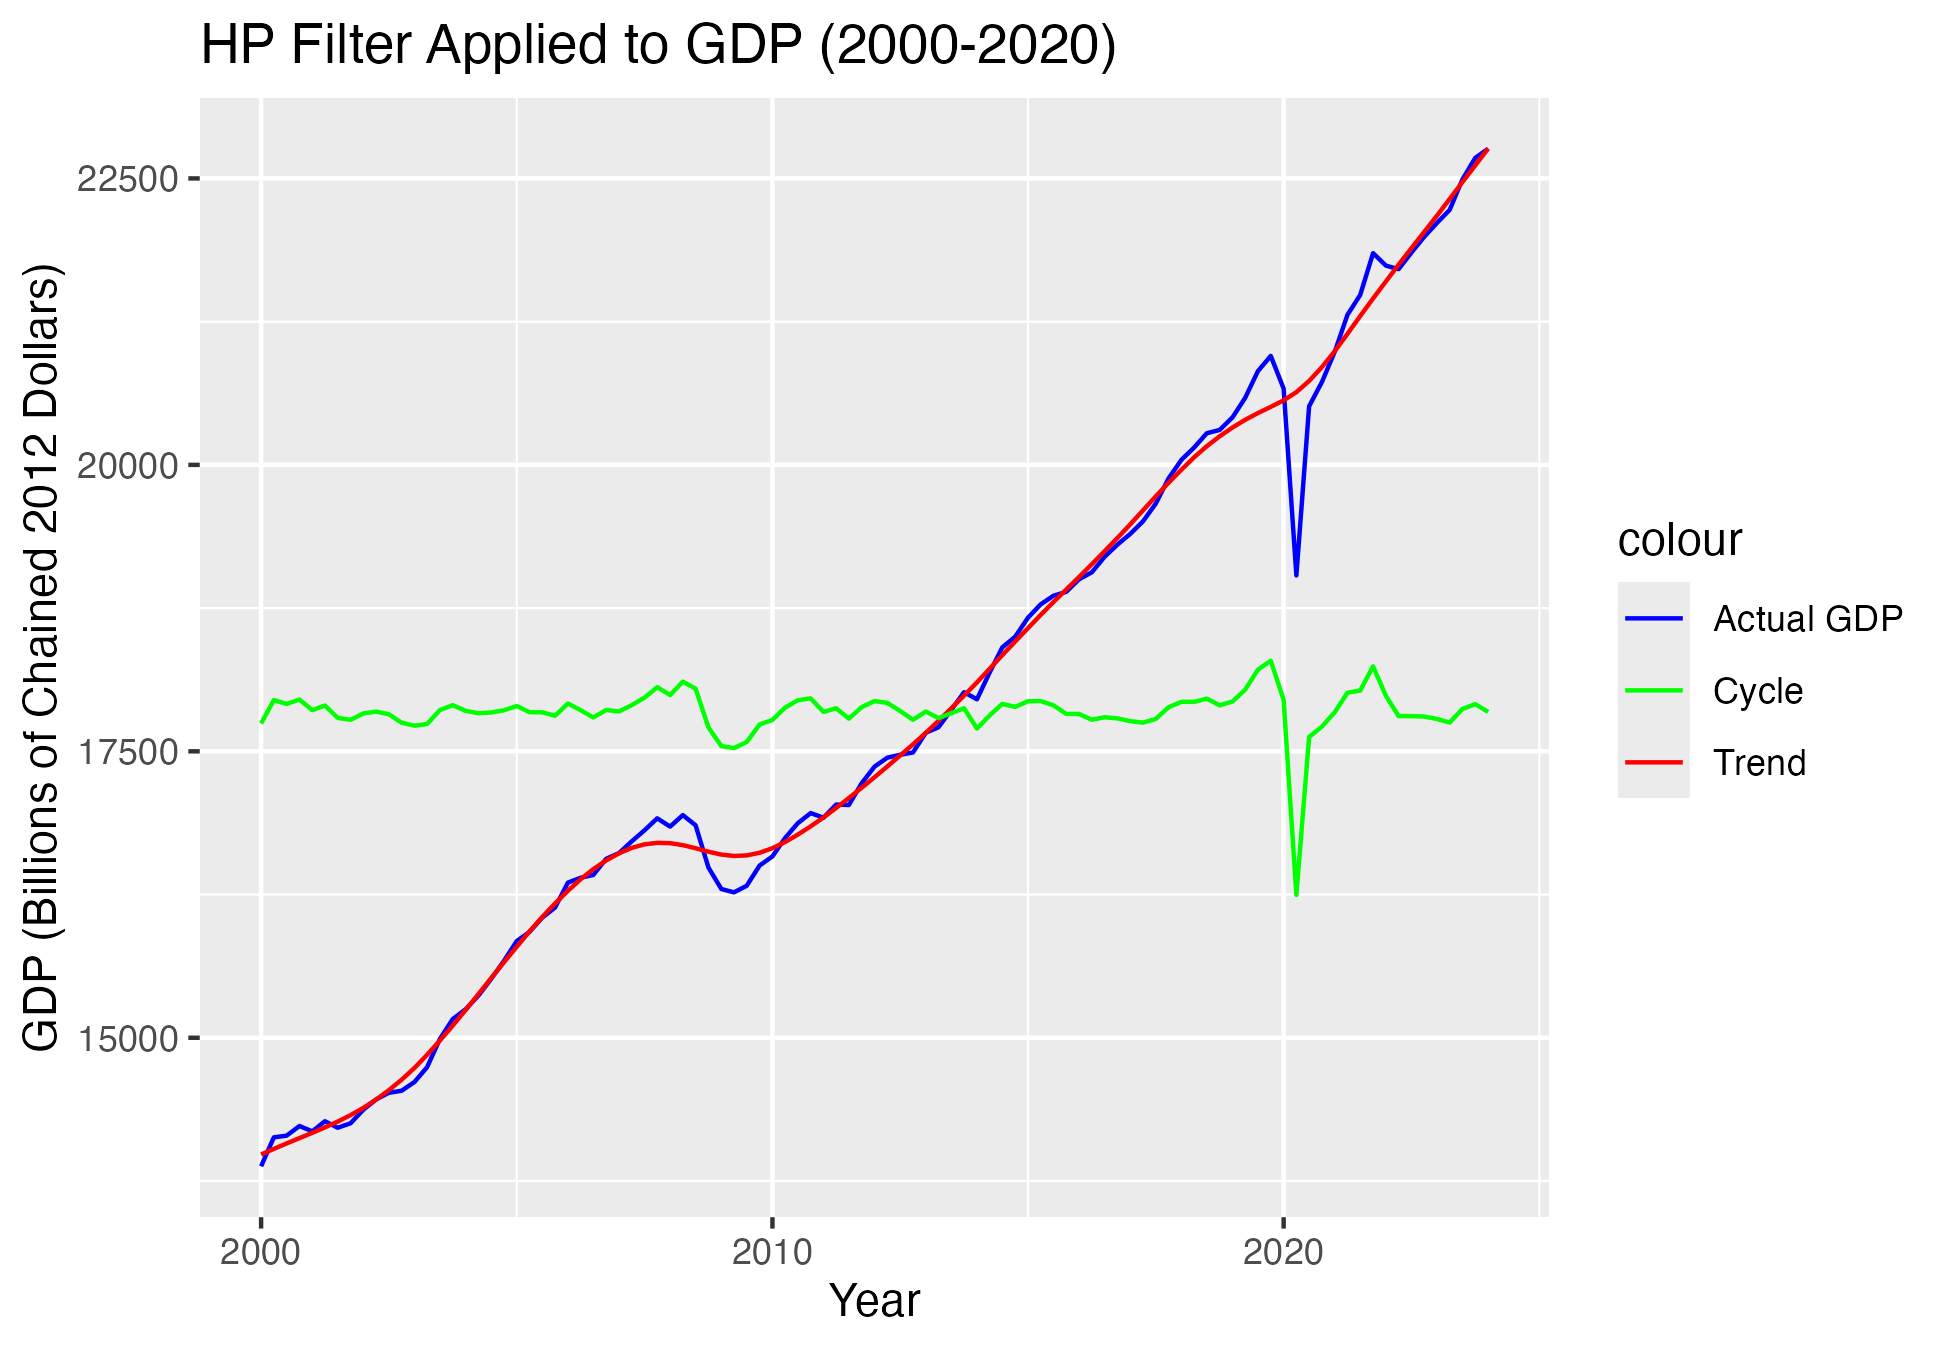
\includegraphics[width=0.9\textwidth]{/Users/cancel/Personal/Coursework/Econ425/VA1/R/HP_Filter_Applied_to_GDP.png}
    \caption{HP Filter Applied to GDP}
\end{figure}

\hrulefill

\section{Conclusion}

Thank you for your attention. This concludes my presentation on macroeconomic concepts. I hope this has provided a clear and comprehensive understanding of the topics. If you have any questions, please feel free to ask.

\end{document}
